\chapter{Main results}
\label{results}

      The result of using the various algoritms FFP6 simulations is shown in Fig(\ref{results}).
We see that our clustering algorithm is better than the one dimensional version \cite{datarishi}.
We hope to compare it with the existing algorithms using FFP6 simulations. We also see that the
neural network method like self organising map with a 200x200 grid performs, very close to the
k-means algorithm where the measures are chosen by hand. It is interesting to note that
\emph{raw-kmeans} performs the same as a self organising map.
\begin{figure}[H]
  \centering
  \label{results}
  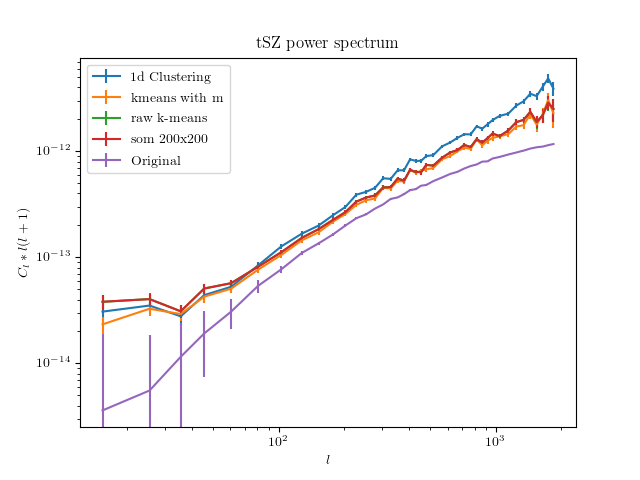
\includegraphics[width=0.7\linewidth]{cl_plots.png}
  \caption{Comparison of the tSZ power spectrum for various methods}
\end{figure}

Seeing that the k-means algorithm using the measures, performs the best out of the various algorithms.
We use that on the frequency maps available on the planck data.

\begin{figure}[H]
  \centering
  \label{results}
  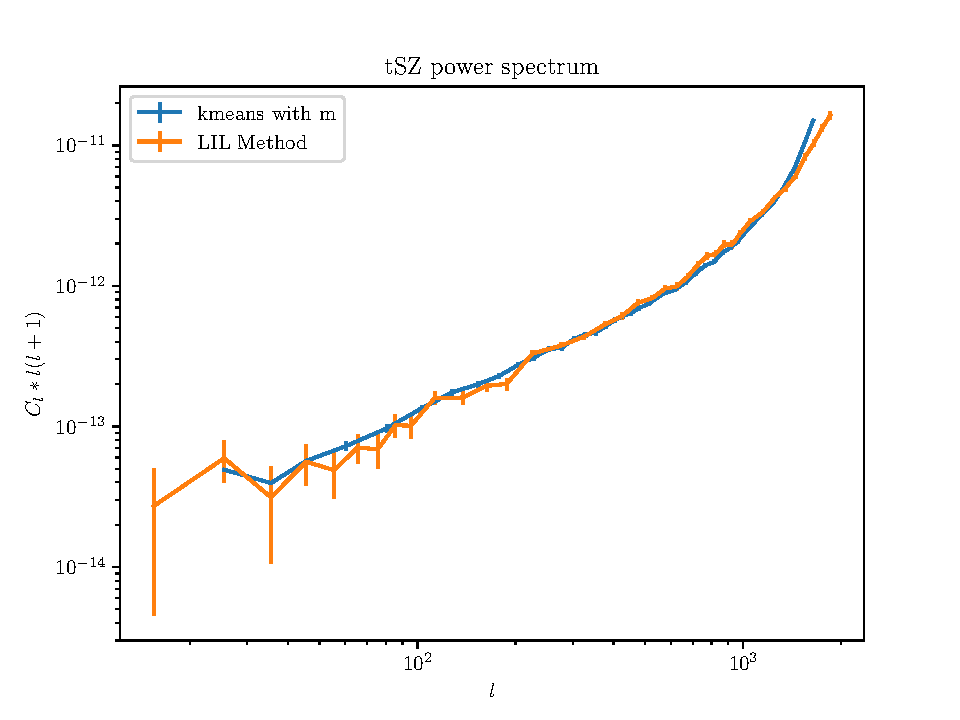
\includegraphics[width=0.7\linewidth]{sz_spec.pdf}
  \caption{Comparison of the tSZ power spectrum of Planck Data using various methods}
\end{figure}

Now, Computing the cross-correlation using the Planck SkyMaps and our own sky maps, We get the following results.
\begin{figure}[H]
  \centering
  \label{results}
  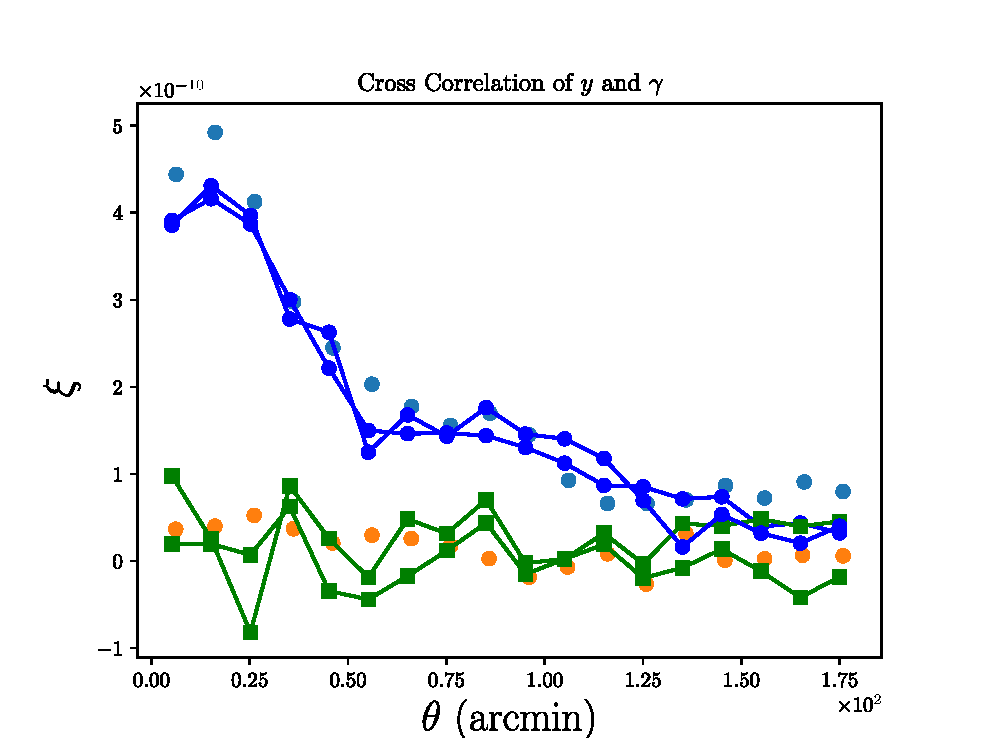
\includegraphics[width=0.7\linewidth]{plot_rcs.eps}
  \caption{Cross Correlation between tSZ and Weak Lensing maps for RCSLens fields}
\end{figure}

\begin{figure}[H]
  \centering
  \label{results}
  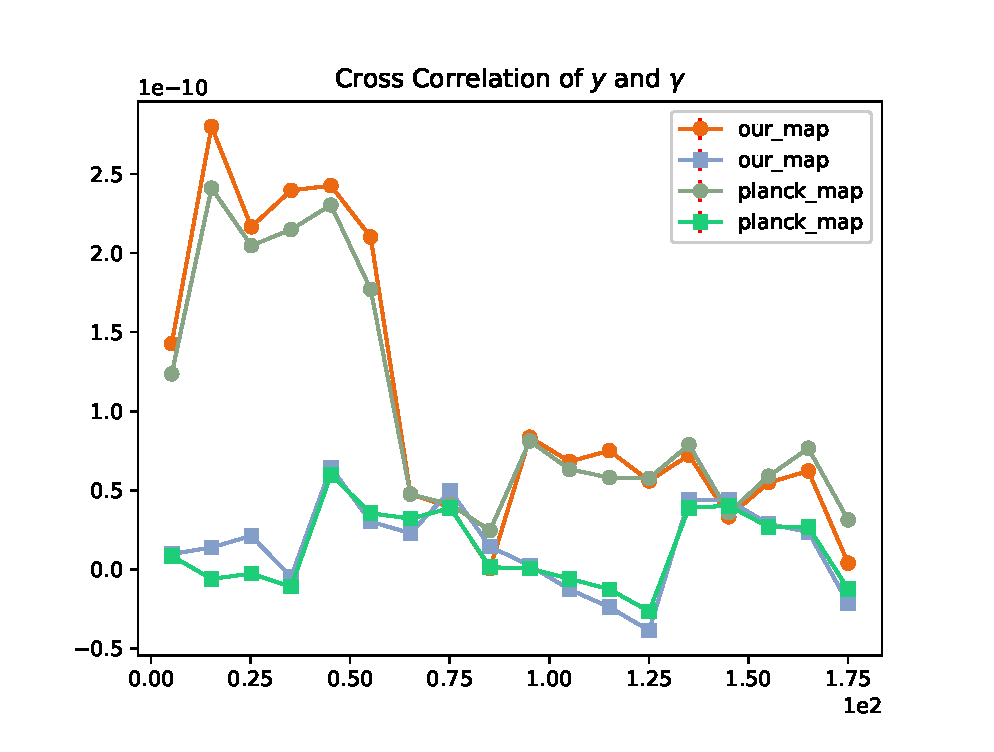
\includegraphics[width=0.7\linewidth]{plot_kids.eps}
  \caption{Cross Correlation between tSZ and Weak Lensing maps for KiDs fields}
\end{figure}

\chapter{ Conclusions}
\label{conc}
      To summarize, We saw that doing foreground clustering using a single measure already
performed on par with the Planck collaboration's pipelines \cite{datarishi}.
We see now that the various machine learning algorithms used for this improves upon the FC-ILC
algorithm using a single measure. We hope that using a independent algorithm to produce maps with
different residuals, would be useful in testing for the effect of foregrounds and any biases in
the existing algorithms for the estimates of the cosmological parameters. We would also like to
point out that in future experiments with more channels using machine learning techniques
with allow for more accuracy than single parameter clustering. 


%%% Local Variables:
%%% mode: latex
%%% TeX-master: "thesis"
%%% End:
